%%-----------------Chapter 6---------------------------
\chapter{Future Efforts and Potential Applications} \labchap{future_efforts}
As you may have noticed, this thesis was an intensive, multi-disciplinary effort that required in-depth knowledge of electronics, board design, software engineering, and systems engineering.
Because of the breadth and depth required by this thesis, some areas were not covered due to technical or temporal constraints.
A large portion of the software was only finalized in the months leading up to finishing this thesis and a hardware fault cost another couple of months of development work.
Therefore, there is a lot left unfinished that is intended for future students to pick up as their own research projects.
Some of these efforts are detailed in this chapter.

\section{Calibration} \labsec{future_calibration}
As discussed at the end of Chapter \ref{chap:calibration}, the calibration procedure failed for the inertial sensors.
The specific reasons could not be determined before the thesis needed to be completed and were out of the technical scope anyways.
Therefore, it will be required in the future to examine these procedures and determine the source of the flaws.

In order to accomplish this, the objective function and constraints should be examined first.
It is likely that the objective function was not used properly with the optimization procedure, producing results that fell into a local minima that satisfied the problem, but did not satisfy the calibration application.
Therefore, the optimization function should be modified to include additional constraints or boundaries to limit the range of ``acceptable'' results from the objective function.
This may improve the accuracy of the calculated misalignment matrices and sensitivity vectors.

Additionally, these procedures should be more thoroughly tested and evaluated across a range of boards and types of sensors.
The calibration script created for this thesis is not sufficient for this task, so the concepts employed by it should be expanded as required.
The measurements can be compared between the boards before and after calibration to determine the efficacy of the proposed procedures.

\section{Hardware Revision F6} \labsubsec{future_hardware}
Based on testing and interviews with Dr. Madgwick \cite{Duffy:2023}, another hardware revision, Revision F6, was created to address some of the concerns with Revision F5.
First, the secondary flash storage chip, the XTSD, was removed entirely since it was redundant and caused the hardware issues that crippled development on Revision F5 for months.

The space created by removing this chip allowed the MARG array to moved to a section of the board that could be mechanically isolated from the rest of the board.
This was necessary because MEMS sensors are affected by strain and in the configuration on Revision F5, the sensors were located at a point of max strain when the board was screwed into the enclosure.
This would affect precision and could cause measurements to slightly vary depending on the torque of the screws used in the assembly.

Additionally, the \lstinline[style=customInline]|data ready| interrupts from the sensors were attached to the microcontroller which should improve performance by switching the measurement method to an interrupt-based one versus polling.
By switching to an interrupt-based measurement method the readings can be taken at a much higher sample rate and be more accurate to the recorded timestamp.
This method is also less computationally intensive on the microcontroller.

Then the microcontroller was changed to one that had an antenna attached directly to its PCB, removing the need for an external antenna.
On the ESP32-S2 microcontroller, the chip would refuse to boot when an external antenna was attached.
This issue was never fully investigated, but the onboard antenna should negate this problem and simplify the overall assembly.

Finally, the power supply was substituted for a more efficient DC-DC converter which should improve efficiency and extend battery life.

This revision has been designed in ECAD, but was not ordered or built due to time constraints.
Therefore, in the future, a student or group of students can build and verify and validate this design using the procedures laid out for Revision F5.

[TODO: Insert picture of Revision F6 and schematic]

\section{Software Improvements} \labsec{future_software}
There are several things that are feasible with the hardware available that were not able to be implemented before the thesis needed to be completed.
Most of these features are not explicitly required by the system requirements, but they could improve the quality and usability of Thetis.
These improvements are being tracked in the Thetis project on GitHub\footnote{\url{https://github.com/users/Legohead259/projects/1}}.

\subsection{Wireless} \labsubsec{future_wireless}
Thetis currently struggles with sending data wirelessly to a host computer.
The only protocol supported is the Universal Datagram Protocol (UDP) which is the simplest internet protocol (IP) to implement.
Packets of data are blasted out with a header denoting the target IP address and port with no regard to signal strength or if the target receives the packet.
This is the most efficient method as there is no handshaking or acknowledgement protocol to saturate the limited bandwidth and compute cycles.

However, as currently implemented, the process takes far to long to format a packet and send it to the target, resulting in a 90\% drop in overall sensor sample rate.
I believe the implementation of the \lstinline[style=customInline]|UDPServer| class is to blame, but more thorough research needs to be performed.
For Thetis to be more effective for the operator, the UDP service should be fixed so that it performs adequately when wirelessly streaming data to a host computer.

Additionally, Thetis cannot handle with the x-IMU3 GUI first connects to it over UDP.
The GUI application broadcasts over 70 requests for settings data simultaneously when first connecting or reading/writing settings which overloads the UDP client buffer on Thetis.
This means that GUI cannot establish proper communication with the device and cannot change settings wirelessly.
Again, to improve its effectiveness and ease of use, this should be fixed.

For deployments, it would also be preferred if the logging and status could be monitored remotely.
This can be done by incorporating a basic web server into Thetis that shows an HTML page with a button for starting/stopping logging and a status box that mimics the on board LED.
Some system information such as time and sensor health could also be presented to the operator for easier diagnostics.
An example can be found in older versions of the firmware.\footnote{\url{https://github.com/Legohead259/ThetisLib/blob/d5982b721212952777a11934ff837b62f7591226/src/radios/wifi.cpp}}.

\subsection{Settings/API} \labsubsec{future_settings}
The settings used on Thetis follow the xioAPI specification which is a set of key/value pairs.
Some of these settings need to be accessible on the device, but should not be overwritten (i.e. factory-settable only).
Currently, Thetis' firmware does not protect these settings and does not support a factory program mode.
This means that at any time, crucial settings like the calibration parameters, serial number, etc. can be overwritten by the user or a host application.
This commonly occurs with the x-IMU3 GUI application which writes blank strings and zero arrays and zero matrices for some factory settings.
When Thetis is connected to the GUI and settings are written to it, a lot of features are temporarily broken until the default values can be restored.
This needs to be fixed to improve the interaction with the operators.

Some settings are also not fully implemented when they should be or they are only implemented at start up.
For example, settings related to sensors such as sensitivity and sample rate are configured when the system first boots.
If these settings are changed during operation, the system must be reset for them to take effect.
This can be streamlined by having callback functions for updating system settings when a new configuration is received.

Several message also need to be implemented, like the battery message.
This will allow the log file to record the battery state over time and may aid with power verification and validation.

\subsection{Data Storage} \labsubsec{future_data}
Currently, the data log recorded to the microSD card is a generic ``logXXX.bin'' where $XXX$ is a three-digit number that is one larger than the previous log file.
While simplistic to implement, this method makes tracking down specific log files difficult as the operator must track the number of times the system is restarted or reset, or the projected length of the log file.
The settings already support custom log file names and prefixes and suffixes, so these should be implemented fully to make logging easier.
Also, the file name extension should be changed to ``.log'' or something similar.

The firmware should also be updated so that the microSD is accessible via different methods.
First, Thetis should show up as a USB flash drive when connected to a host computer.
Files can be transferred over the USB connection without removing the microSD card.
Second, the filesystem should be accessible over a FTP service where operators can wirelessly log in and copy/remove files.
This will be very useful for deployed applications where Thetis cannot be easily opened or physically accessed.

\subsection{Sensors} \labsubsec{future_sensors}
Many of the sensors implemented in the firmware are based upon the Adafruit libraries for those components.
While this simplifies the integration, it bloats the memory and storage requirements.
This also creates a dependency on third-party software which could be problematic in some situations.
Therefore, it would be nicer to have all of the sensors packaged individually in libraries that are self-contained and conform to the I2CDevLib\footnote{\url{https://www.i2cdevlib.com/}} standards.
This would improve the code performance and reduce memory requirements.

Additionally, the \lstinline[style=customInline]|Fusion| library has implemented some new features for accelerometer and magnetometer rejection and status flags that would be useful for the entire sensor fusion process.
Therefore, the firmware should be migrated to this new version and have these features implemented.

If the hardware is migrated to Revision F6, the sensor polling method should also be swapped out for an interrupt-based approach.
Instead of asking the sensors every period what their data is, the method must change to asking as soon as a pulse is received on the ``data ready'' input pins.
This will make computation more efficient and allow for high sampling speeds.
Also, the divisor settings can be implemented here to automatically average $N$ number of samples before reporting it.

\section{More Verification and Validation} \labsec{future_vv}
Identifying and fixing a major design flaw with Thetis Revision F5 occupied a large amount of time that could have been used to further verify and validate some features.
Unfortunately, that means there are still some things to be analyzed before the design can be considered ``100%'' completed.

\subsection{Wireless} \labsubsec{future_vv_wireless}
The wireless features of Thetis need to verified by proving that data and settings can be streamed from the device to the host computer over a UDP connection.
This should be done in both access point and client modes to cover the breadth of use cases.
Of course, before these tests can be done, the problem with the UDP server and client should be addressed.

It is also important to characterize the strength, speed, and bandwidth to understand the limits of the wireless features.
To test the signal strength, Thetis should be enclosed in its container and then set to wireless access point mode.
A smartphone with the appropriate application can then detect the Thetis access point and will report its strength.
Move the phone several distances away from the access point and plot to get a rough characteristic.

Similarly, Thetis can be placed into the wireless client mode and connected to a local access point.
Assuming the message is implemented in the firmware, Thetis can report the wireless signal strength and log it.
Again, move Thetis given distances away from the access point and plot to roughly characterize it.
The connection speed and bandwidth can be tested by running files of a known size through the FTP service and recording the amount of time to transfer the data.
Ideally, there will be decent strength out to about 10-meters and the file transfers will occur within a minute or two.

\subsection{Power} \labsubsec{future_vv_power}
The verification and validation for power described in this thesis was just ``does it last four hours or not''.
It is important to fully characterize the power draw so that the operator can know the limits of the device.
Additionally, measuring the power draw during certain operation modes can identify points for improvement and the hardware or software can be modified to increase battery life.
The devices can also be put into a sleep mode (assuming that is supported in the firmware) and power consumption characterized.
With the normal operating mode and sleep mode consumptions known, it will be possible to set up a burst measurement mode to increase deployment life, if desired.

\section{Calibration Machine} \labsec{future_calibration_machine}
Calibrating Thetis is currently a manual process that is prone to errors from the procedure and the testing apparatus.
For example, in the gear apparatus for calibrating the accelerometer and orientation, the calibration cube could accidentally be misplaced by a single tooth, causing a deviation of 5-degrees.
This may not be immediately caught, introducing errors.
To automate the process and reduce potential errors, an expansion upon the current calibration machine is proposed which incorporates more features to improve usability.

\subsection{Requirements} \labsubsec{future_cm_requirements}
In order to effectively automate the process and reduce the chances of human error, the machine should be able to rotate the IMU about all three-axis on its own and in a controlled manner.
Additionally, each of these rotations should be tracked with an absolute position sensor to understand the IMU's position and rotational velocity to a high degree of accuracy.
The most compact way to accomplish this may be to borrow the design from a three-axis camera gimbal using high torque brushless DC motors, as shown in Figure \ref{fig:three_axis_gimbal}.

\begin{figure}
    \centering
    \caption[Three Axis Gimbal]{The rear of a three-axis gimbal used on UAVs for action cameras. 
    Courtesy of RC Product India. \url{https://www.rcproduct.in/product/feiyutech-oem-sftuav-mini-3d-3-axis-gimbal/}}
    \labfig{three_axis_gimbal}
    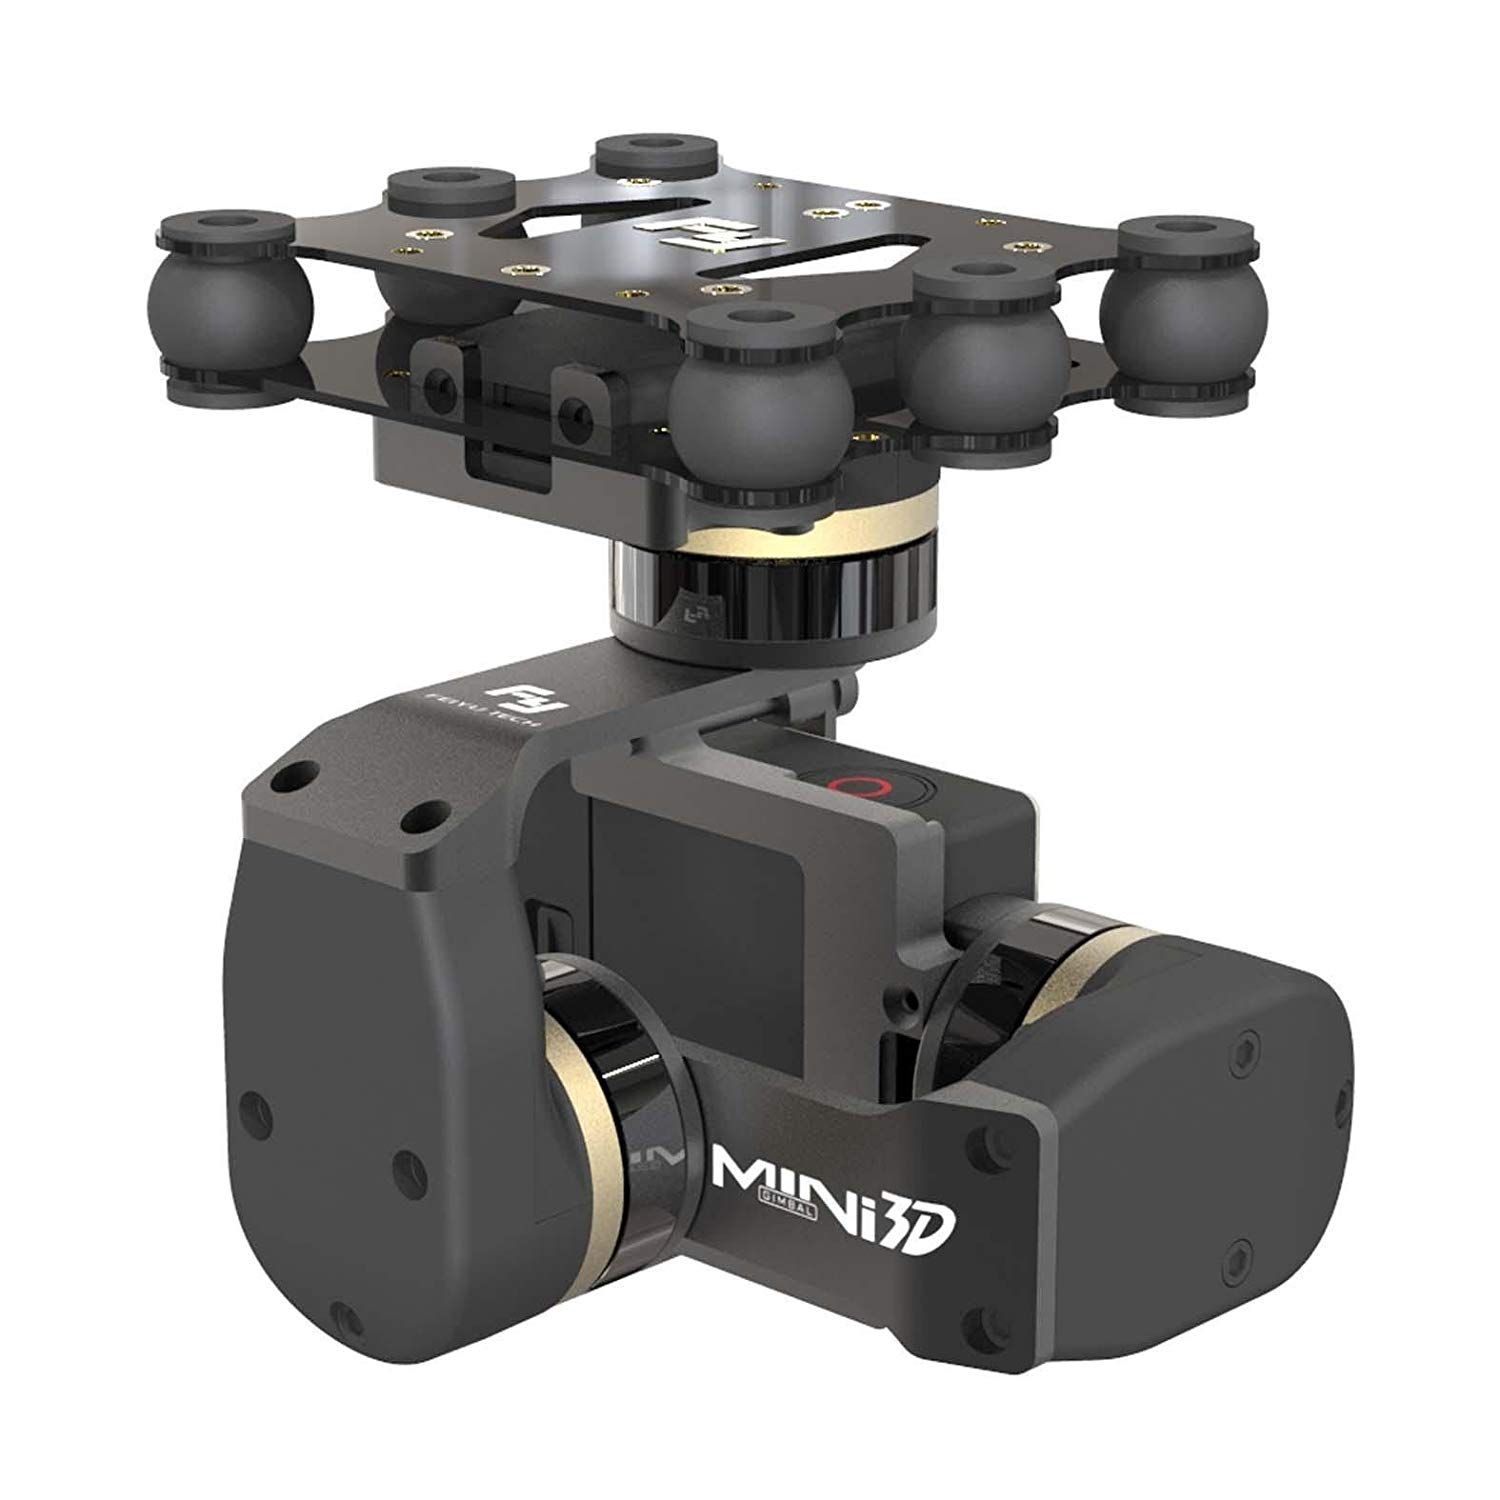
\includegraphics[height=2in]{future_efforts/three-axis-gimbal.png}
\end{figure}

Controls for the motor need to happen in near real-time and the main computer should also be able to send commands and data around the system quickly and efficiently.
This can be accomplished with a Data Distribution Service (DDS) topology that incorporates publish/subscribe and client/server interactions.
The most popular framework for this type of network is ROS2, which is used on the current calibration machine and should be able to modified to a new platform.
The new calibration machine should also be open architecture such that new IMUs with different communication methods or new calibration sensors can be quickly integrated.

Finally, the main controller for the new machine should be powerful enough and have enough storage access to build a database with the calibration and validation results.
Ideally, this controller would also have access to the Internet so that the information could be published to a cloud database for more accessibility.
It would also be prudent to have the controller in a headed configuration with a simple touchscreen user interface to start/stop the procedure and monitor the system status.

\subsection{Block Diagram} \labsubsec{future_cm_block_diagram}
To meet the proposed requirements, the hardware block diagram in Figure \ref{fig:calibration_machine_v2} is introduced.
The core of the machine is a Raspberry Pi microcomputer that would be running Ubuntu with ROS2 loaded onto it.
A Hardware Attached on Top (HAT) daughter board would be attached and responsible for handling the sensor inputs, motor driving, etc.
The Pi would be connected to an official 7-inch touchscreen as a human-machine interface (HMI) and then connected to a local area network (LAN) for connectivity features.

The motors for the gimbal would have a diametrically magnetized magnet on the shaft with a magnetic compass placed beneath it.
As the magnet moves, the compass can detect the rotation direction and speed.
By determining a ``home'' position, the compass can also detect the degrees rotated from an arbitrary zero point.
This allows ground truth measurements to be taken for the gyroscope, accelerometer, and orientation datasets for all three rotation axes.
A microcontroller can be placed on the Raspberry Pi HAT and handle the real-time control of the motors and sensors, while interfacing with the Pi over a serial port such as UART, SPI, or I2C.

[TODO: Insert block diagram for calibration machine]

The data can be run through the ROS2 packages and a master script can analyze the data at the end of the calibration process and produce the results.
Then, the same can occur after the validation process and a calibration certificate can be made that shows the IMU error over all the testing regimes.
This architecture is represented in the block diagram in Figure \ref{fig:calibration_machine_ros}.

[TODO: Insert block diagram for the ROS2 architecture]

\subsection{Concept of Operations} \labsubsec{future_cm_conops}
For the new calibration machine, the idea is a one-touch solution that is fully automated, requiring minimal human intervention.
At the start of the test, the operator can press the ``Start'' button and the machine will home each axis to a zero point and begin calibrating the accelerometer and gyroscope.
Each axis will be individually rotated in 45-degree increments for a complete revolution.
Then, they will be rotated at a few target speeds.
Simultaneously, the IMU will be streaming data to the Raspberry Pi for collection and processing.
After the accelerometer and gyroscope datasets are collected, the IMU will be simultaneously rotated about all three axes to collect the magnetometer calibration dataset.

When these steps are completed, the master script will compute the calibration parameters and upload them to the IMU's sensor fusion algorithm.
Then, restart the testing procedure with finer increments to increase the number of validation data points collected.
After the sensor validation datasets are collected, the machine will rotate the IMU into various poses as part of the orientation validation dataset.
Finally, the master script will process the validation datasets into a single calibration certificate product that the operator can view.

While the entire process is occurring, crucial data will be shown on the screen to the operator along with an ``ESTOP'' button.
If the machine detects an error, or the human operator wants to stop the test, there will be a set of commands to safely shutdown the system.
Additionally, the machine will have several settings that can be tweaked by the operator prior to a calibration run - like the gimbal zero positions.

\section{Floating Body Testing} \labsec{future_testing}
The original intent of Thetis was to supplement class resources in the Ocean Engineering department.
Naturally, this means that Thetis should be used in Ocean Engineering applications by students.
Instructors may also find Thetis useful for their research as it is a small and cheap platform, perfect for a proof of concept experiment that could lead to larger revelations.

\subsection{Surfboard} \labsubsec{future_testing_surf}
The first application is in the Surf Engineering Analysis or Ocean Engineering Data Analysis course.
Here, students will put Thetis into a surfboard and paddle out into the ocean surf to catch some waves.
Thetis' sensor suite will provide students data on the board's orientation, acceleration, velocity, and position in the local and global coordinate frames which they can use as part of their class project.
Thetis improves upon the sensors used for that course by having a larger sensor suite and a better sensor fusion algorithm to process the data.
It would also be interesting to put the x-IMU3 into the same board and environment and see how they compare.

\subsection{Model Barge} \labsubsec{future_testing_barge}
Another application is with the fluids laboratory or a naval architecture laboratory section.
Currently, one lab experiment performed by students is the analysis of a vessel's movement based on weight placement and metacentric height.
The model barge is equipped with inclinometers for the pitch and roll that students must analyze time step by time step to create a plot of the roll/pitch.
Typically, this is done after the experiment doing frame-by-frame video analysis.
If the video is blurry, or the vessel yaws during the test, this analysis can be difficult and time-consuming.

To simplify the process, Thetis can be placed on the barge and set to record the vessel's orientation at a much high frequency than a frame-by-frame analysis and more accurately.
The data can also be stream wireless in real-time to a host computer that would allow the instructor to more dynamically and visually demonstrate the effect of metacentric height on vessel stability.
This can also be done to larger scale vessels in a larger tank or in a class room.

\subsection{WEAVE} \labsubsec{future_testing_weave}
The last major application considered is the proposed Wave Estimating Algorithm for Vessels Experiment, or WEAVE.
Based on the floating model barge experiments and previous work done in \cite{Gait-Tracking}, WEAVE is an exciting study into an alternative method for wave characteristic measurement.
Thetis can be placed on top or within a wave buoy and deployed on the ocean.
While there, it can record the inertial characteristics of the buoy which can be used to determine the wave parameters over time.
The parameters can be calculated in both the time and frequency domains which would be compared to the ground truth from the wave buoy.
For more information, a more in-depth whitepaper manuscript is presented in Appendix \ref{chap:weave}.